%% LyX 2.1.1 created this file.  For more info, see http://www.lyx.org/.
%% Do not edit unless you really know what you are doing.
\documentclass[twocolumn,pre, reprint, nofootinbib]{revtex4-1}
\usepackage[latin9]{inputenc}
\setcounter{secnumdepth}{3}
\usepackage{amssymb}
\usepackage{graphicx}
\usepackage{amsmath}
\usepackage{hyperref}


\newcommand\blfootnote[1]{%
  \begingroup
  \renewcommand\thefootnote{}\footnote{#1}%
  \addtocounter{footnote}{-1}%
  \endgroup
}
\makeatletter

%%%%%%%%%%%%%%%%%%%%%%%%%%%%%% LyX specific LaTeX commands.
%% Because html converters don't know tabularnewline
\providecommand{\tabularnewline}{\\}

%%%%%%%%%%%%%%%%%%%%%%%%%%%%%% Textclass specific LaTeX commands.
% Fix a couple of bugs in REVTeX 4.1
\def\lovname{List of Videos}
\@ifundefined{textcolor}{}
{
 \definecolor{BLACK}{gray}{0}
 \definecolor{WHITE}{gray}{1}
 \definecolor{RED}{rgb}{1,0,0}
 \definecolor{GREEN}{rgb}{0,1,0}
 \definecolor{BLUE}{rgb}{0,0,1}
 \definecolor{CYAN}{cmyk}{1,0,0,0}
 \definecolor{MAGENTA}{cmyk}{0,1,0,0}
 \definecolor{YELLOW}{cmyk}{0,0,1,0}
}

\makeatother

\begin{document}

\title{Anti-ferromagnetic Ising Model in Hierarchical Networks }


\author{Xiang Cheng and Stefan Boettcher}

\affiliation{Department of Physics, Emory University, Atlanta, GA 30322, USA}
\begin{abstract}
The Ising antiferromagnet  is a convenient model of glassy dynamics.  It can introduce geometric frustrations and may give rise to a spin glass phase and glassy relaxation at low temperatures.  We apply the antiferromagnetic Ising model to 3 hierarchical networks which share features of both small world networks and regular lattices. Their recursive and fixed structures make them suitable for exact renormalization group analysis as well as numerical simulations. We first explore the dynamical behaviors using simulated annealing and discover an extremely slow relaxation at low temperatures. Then we employ the Wang-Landau algorithm to investigate the energy landscape and the corresponding equilibrium behaviors for different system sizes. Besides the Monte Carlo methods, renormalization group is used to study the equilibrium properties in the thermodynamic limit and to compare with the results from simulated annealing and Wang-Landau sampling. 
\smallskip 
\end{abstract}

\maketitle

\section{Introduction}

\label{sec:intro} 
The Ising antiferromagnet can introduce geometric frustrations and may give rise to interesting dynamics and phases. What may make it more interesting is applying the antiferromagnetic model to hierarchical networks which have a lattice backbone and small-world structure. These networks could produce different critical phenomena from that found on lattice geometries \cite{boettcher15epl}.

\section{RG Calculations}
\label{sec:RG}
 The setup of renormalization is started by separating the Ising Hamiltonian into hierarchies
\begin{equation}
-\beta\mathcal{H} = \sum_{n=1}^{k-2} (-\beta \mathcal{H}_n)+ \mathcal{R}(K_2, K_3, \cdots)
\end{equation}
where $\mathcal{R}$ is the coupling beyond $\mathcal{H}_n$ of levels $k>2$. $\mathcal{H}_n$ depends on the interactions $K_0$ on the backbone and $L_0$, $L_1$, $K_1, \cdots$ among the long range couplings. We describe the RG procedure network by network. 

\subsection{Ising antiferromagnet on HN3 and HN5}
\label{sec:hn35rgafm}
The Hamiltonian with magnetic field is
\begin{eqnarray}
\label{eq:hpz0}
 -\beta \mathcal{H}_n &=& K_0 \left(x_{n-2}x_{n-1} + x_{n-1}x_{n} +  x_{n}x_{n+1} +  x_{n+1}x_{n+2}\right) \nonumber \\ 
   && + K_1(x_{n-1}x_{n+1}) + yL_1(x_{n-2} x_{n+2}) \nonumber \\
   && +L_0(x_{n-2}x_{n} + x_{n}x_{n+2})  + 4I \nonumber\\
   && +\frac{H_K}{2}(x_{n-2} + 2x_{n-1}+2x_n+2x_{n+1}+x_{n+2})\nonumber\\
   && +\frac{H_L}{2}(x_{n-2}+2x_n + x_{n+2}) + \frac{H}{2}(x_{n-1}+x_{n+1})\nonumber\\
   && + \frac{T}{2}(x_{n-2}x_{n-1}x_n + x_n x_{n+1} x_{n+2})
\end{eqnarray}
where $y=0$ for HN3 and $y=1$ for HN5.
In the RG process of antiferromagnetic Ising model, one of the major differences is definition of $\mu$. The reduced temperature is defined as
\begin{equation}
\mu = \exp[\frac{2}{T}]
\end{equation}
where $T$ is the temperature. Thus, $\mu \ge 1$, and
\begin{align*} 
T \rightarrow 0 :  \mu \rightarrow \infty : \frac{1}{\mu}\rightarrow 0_+  \\ 
T \rightarrow \infty :  \mu \rightarrow 1_+ : \frac{1}{\mu}\rightarrow 1_-
\end{align*}



\subsubsection{Internal Energy of HN3}
The ground state energy is 
\begin{equation}
GS_{HN3} = -1
\end{equation}
See the Figure \ref{fig:h3erg} and \ref{fig:h3ergmc} for results.
\begin{figure}[!h]
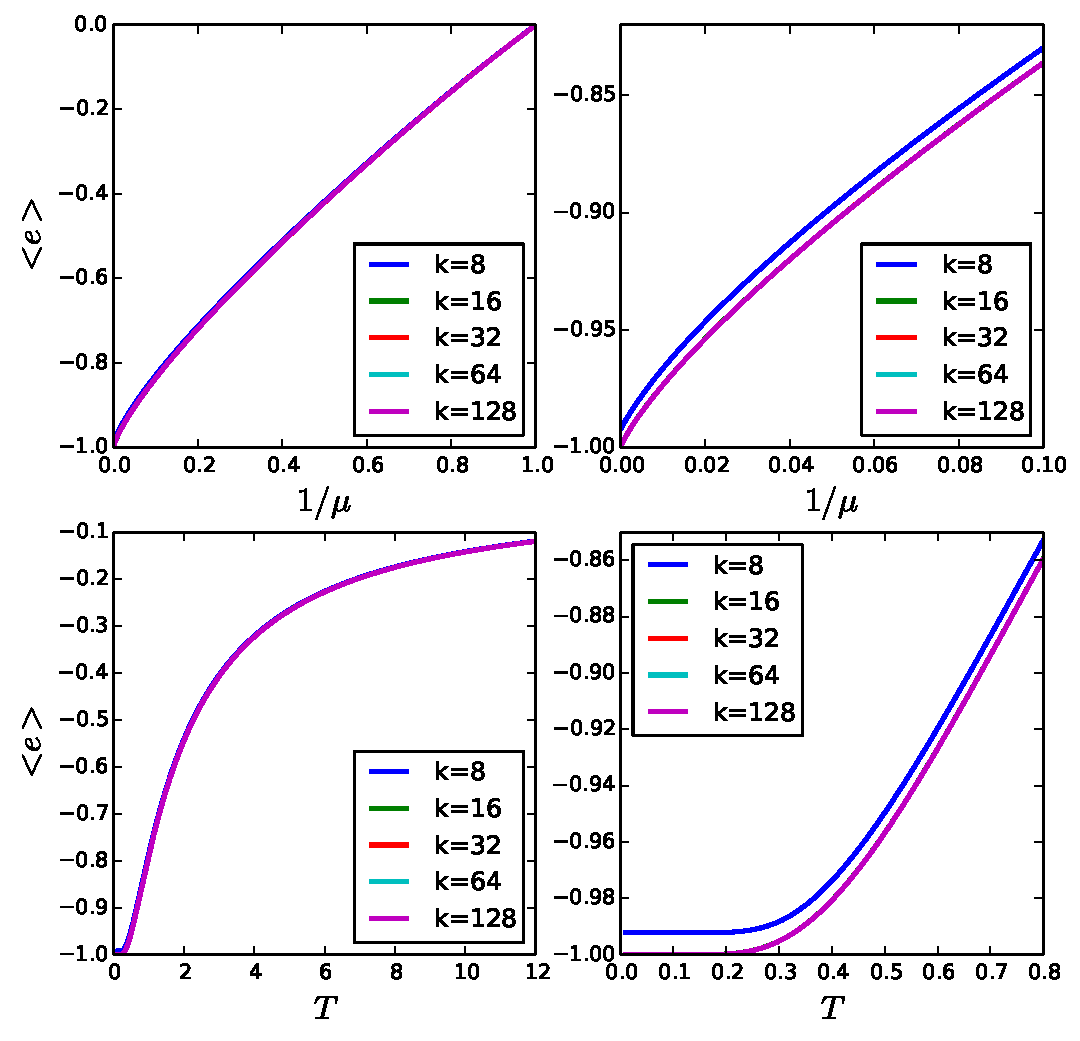
\includegraphics[width=1\columnwidth]{../RG_plots/HN3_IE_rg.pdf}
\caption{HN3 Ising AFM Internal Energy vs temperature.}
\label{fig:h3erg}
\end{figure}
\begin{figure}[!h]
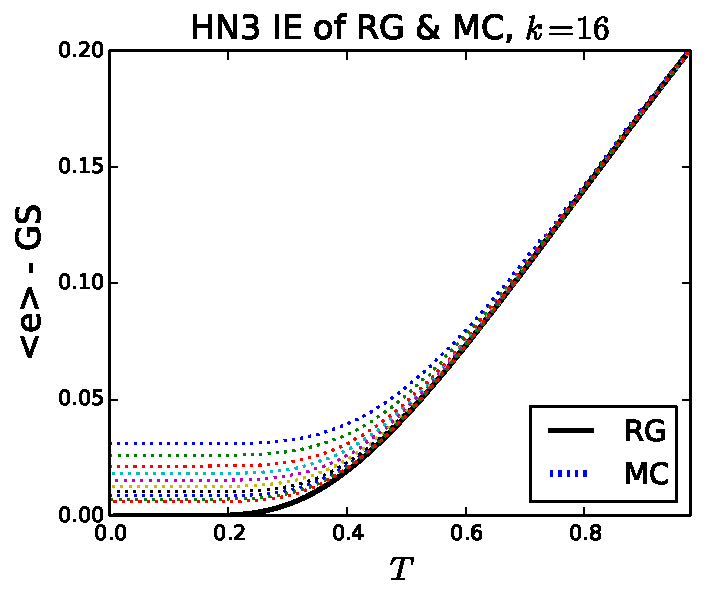
\includegraphics[width=1\columnwidth]{../RG_plots/HN3_IE_rgmc.pdf}
\caption{HN3 Ising AFM Internal Energy from RG and MC.}
\label{fig:h3ergmc}
\end{figure}

\subsubsection{Internal Energy of HN5}
The ground state energy for $N\rightarrow\infty$ is 
\begin{equation}
GS_{HN5} = -\frac{7}{6}=-1.166666666\dotsc
\end{equation}
See the Figure \ref{fig:h5erg} and \ref{fig:h5ergmc} for results.
\begin{figure}[!h]
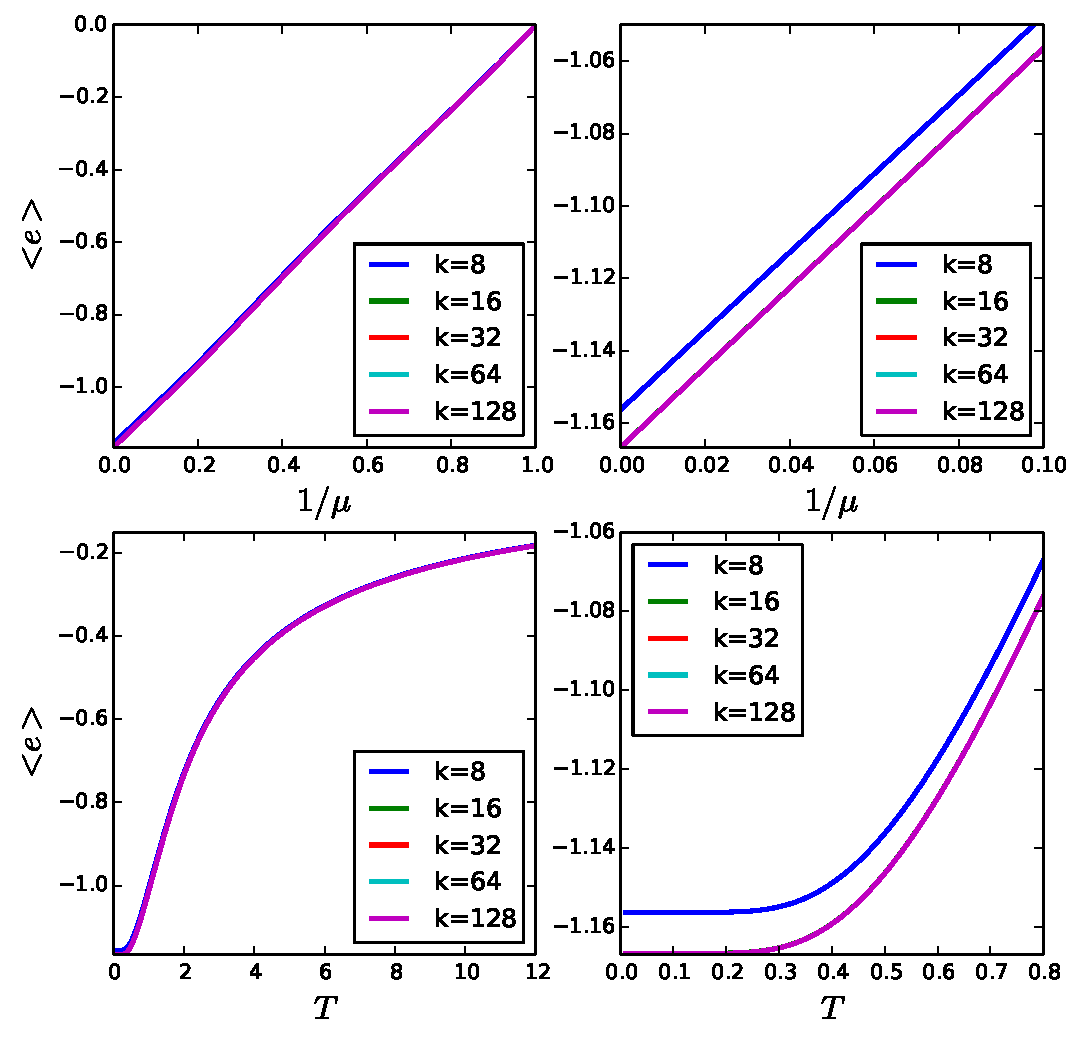
\includegraphics[width=1\columnwidth]{../RG_plots/HN5_IE_rg.pdf}
\caption{HN5 Ising AFM Internal Energy vs temperature.}
\label{fig:h5erg}
\end{figure}

\begin{figure}[h]
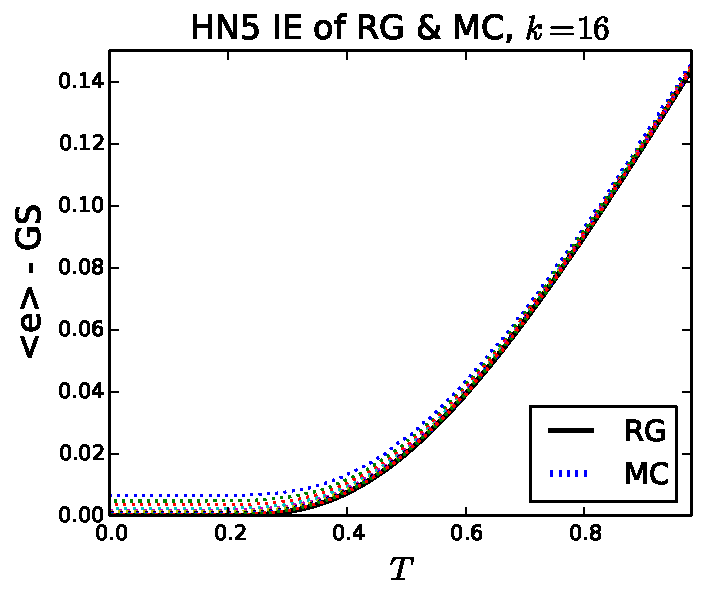
\includegraphics[width=1\columnwidth]{../RG_plots/HN5_IE_rgmc.pdf}
\caption{HN5 Ising AFM Internal Energy from RG and MC.}
\label{fig:h5ergmc}
\end{figure}


\subsubsection{ Magnetization of HN3}
\textbf{\emph{Magnetization vs. big H}}\\
This part is to learn how $<m>$ changes with $H$, which shows a different phenomena as shown in Figure \ref{fig:h3mhrg}.
\begin{figure}[!htbp]
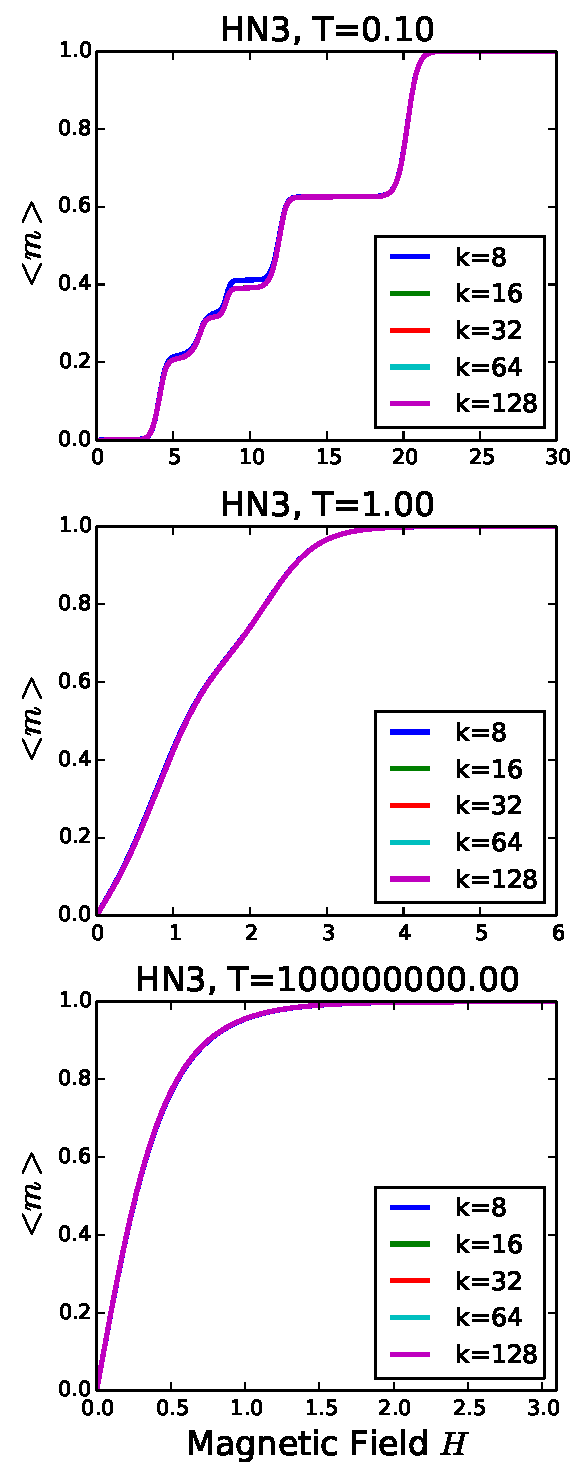
\includegraphics[width=0.8\columnwidth]{../RG_plots/HN3_MagH_rg_v2.pdf}
\caption{HN3 Ising AFM magnetization vs magnetic field from RG. $H$ in the RG is actually reduced magnetic field, i.e. $H/T$.}
\label{fig:h3mhrg}
\end{figure}
\\


\subsubsection{ Magnetization of HN5}
\textbf{\emph{Magnetization vs. big H}}\\
This part is to learn how $<m>$ changes with $H$, which shows a different phenomena as shown in Figure \ref{fig:h3mhrg}.
\begin{figure}[!htbp]
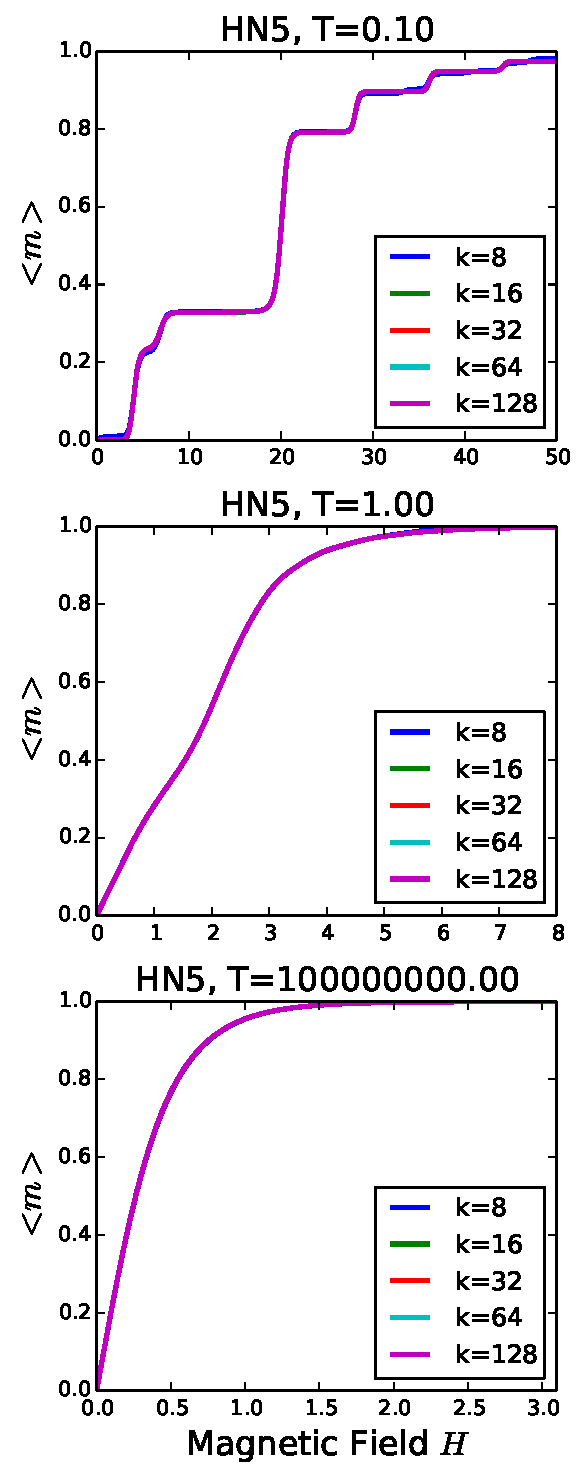
\includegraphics[width=0.8\columnwidth]{../RG_plots/HN5_MagH_rg_v2.pdf}
\caption{HN5 Ising AFM magnetization vs magnetic field from RG. $H$ in the RG is actually reduced magnetic field, i.e. $H/T$.}
\label{fig:h5mhrg}
\end{figure}
\\


\subsubsection{Specific Heat of HN3}
See Figure \ref{fig:h3cvrg} for results.

\begin{figure}[!htb]
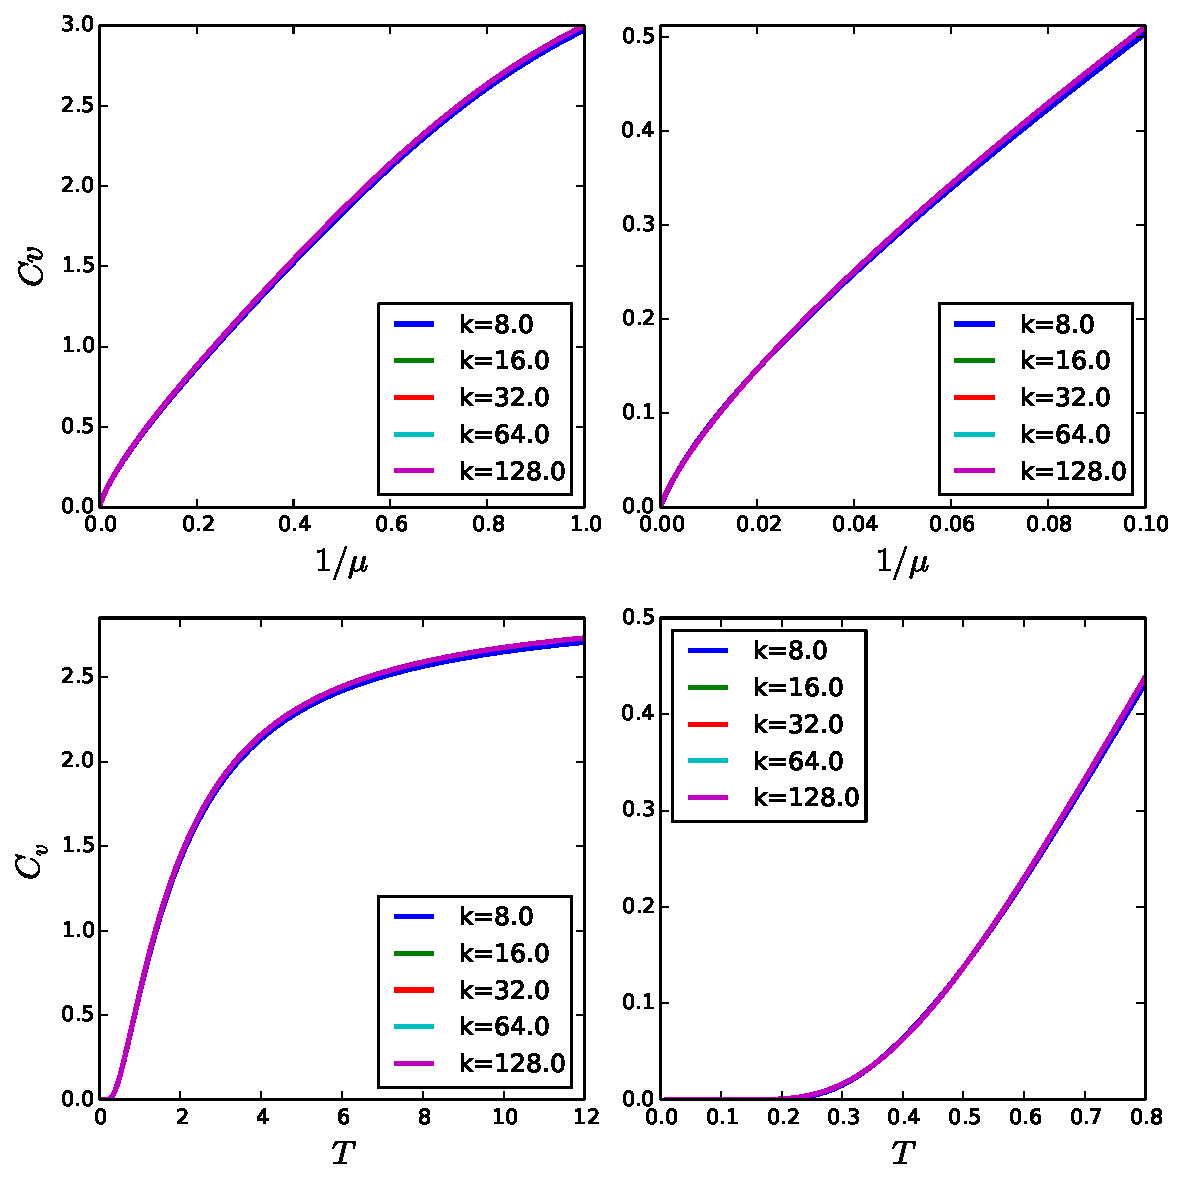
\includegraphics[width=1\columnwidth]{../RG_plots/HN3_Cv_rg_v2.pdf}
\caption{HN3 Ising AFM Specific Heat from RG.}
\label{fig:h3cvrg}
\end{figure}


\subsubsection{Specific Heat of HN5}
See Figure \ref{fig:h5cvrg} for results.

\begin{figure}[!htb]
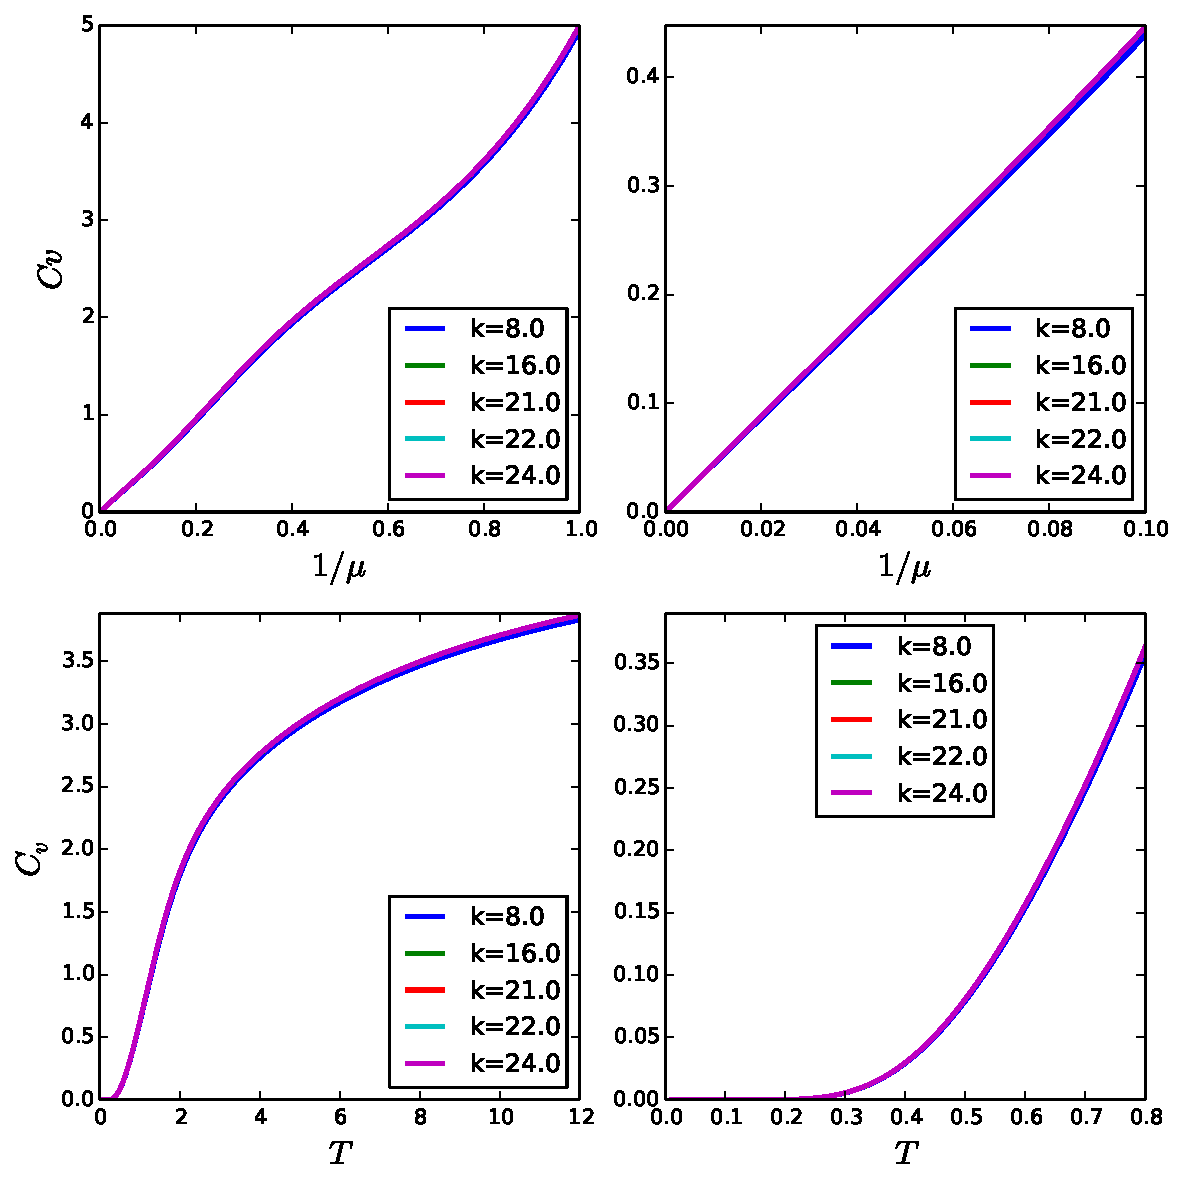
\includegraphics[width=1\columnwidth]{../RG_plots/HN5_Cv_rg_v2.pdf}
\caption{HN5 Ising AFM Specific Heat from RG.}
\label{fig:h5cvrg}
\end{figure}

\subsubsection{Susceptibility of HN3}
See Figure \ref{fig:h3xrg} for results.
\begin{figure}[!htbp]
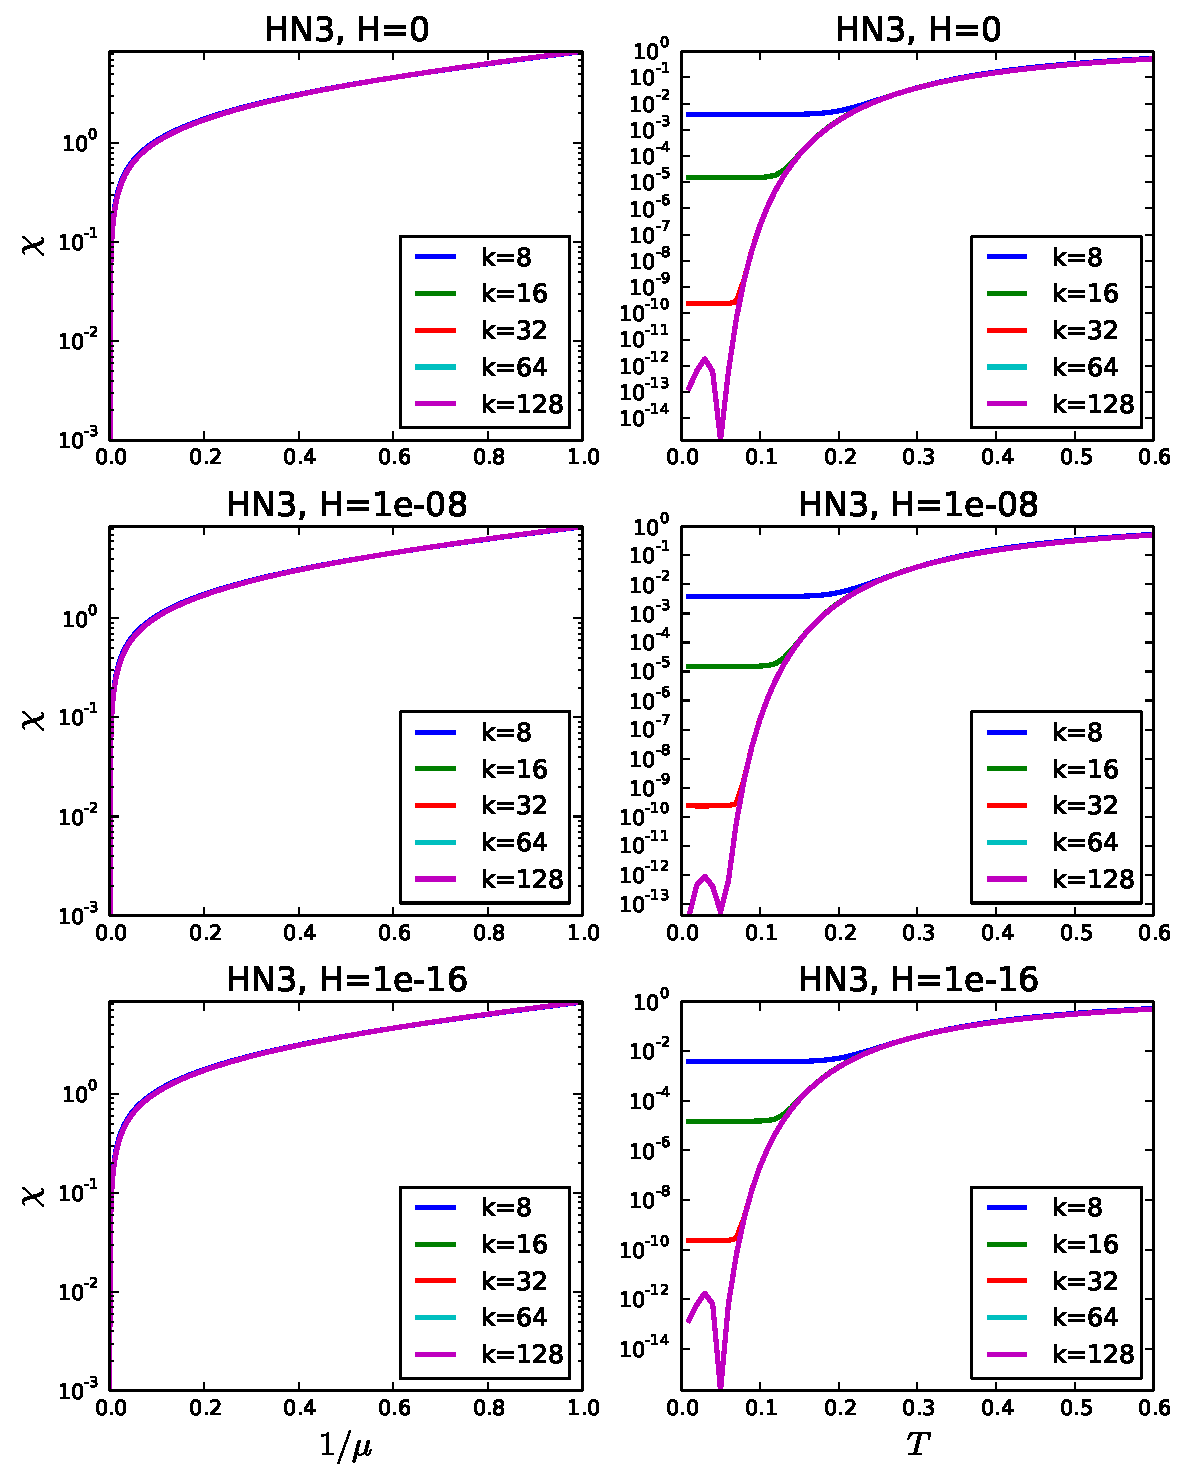
\includegraphics[width=1\columnwidth]{../RG_plots/HN3_XT_rg.pdf}
\caption{HN3 Ising AFM  Susceptibility from RG. The precision of RG is already N[1000].  I may try smaller T step size at low T to improve the accuracy at low $T$.}
\label{fig:h3xrg}
\end{figure}

\subsubsection{Susceptibility of HN5}
See Figure \ref{fig:h5xrg} for results.
\begin{figure}[!htbp]
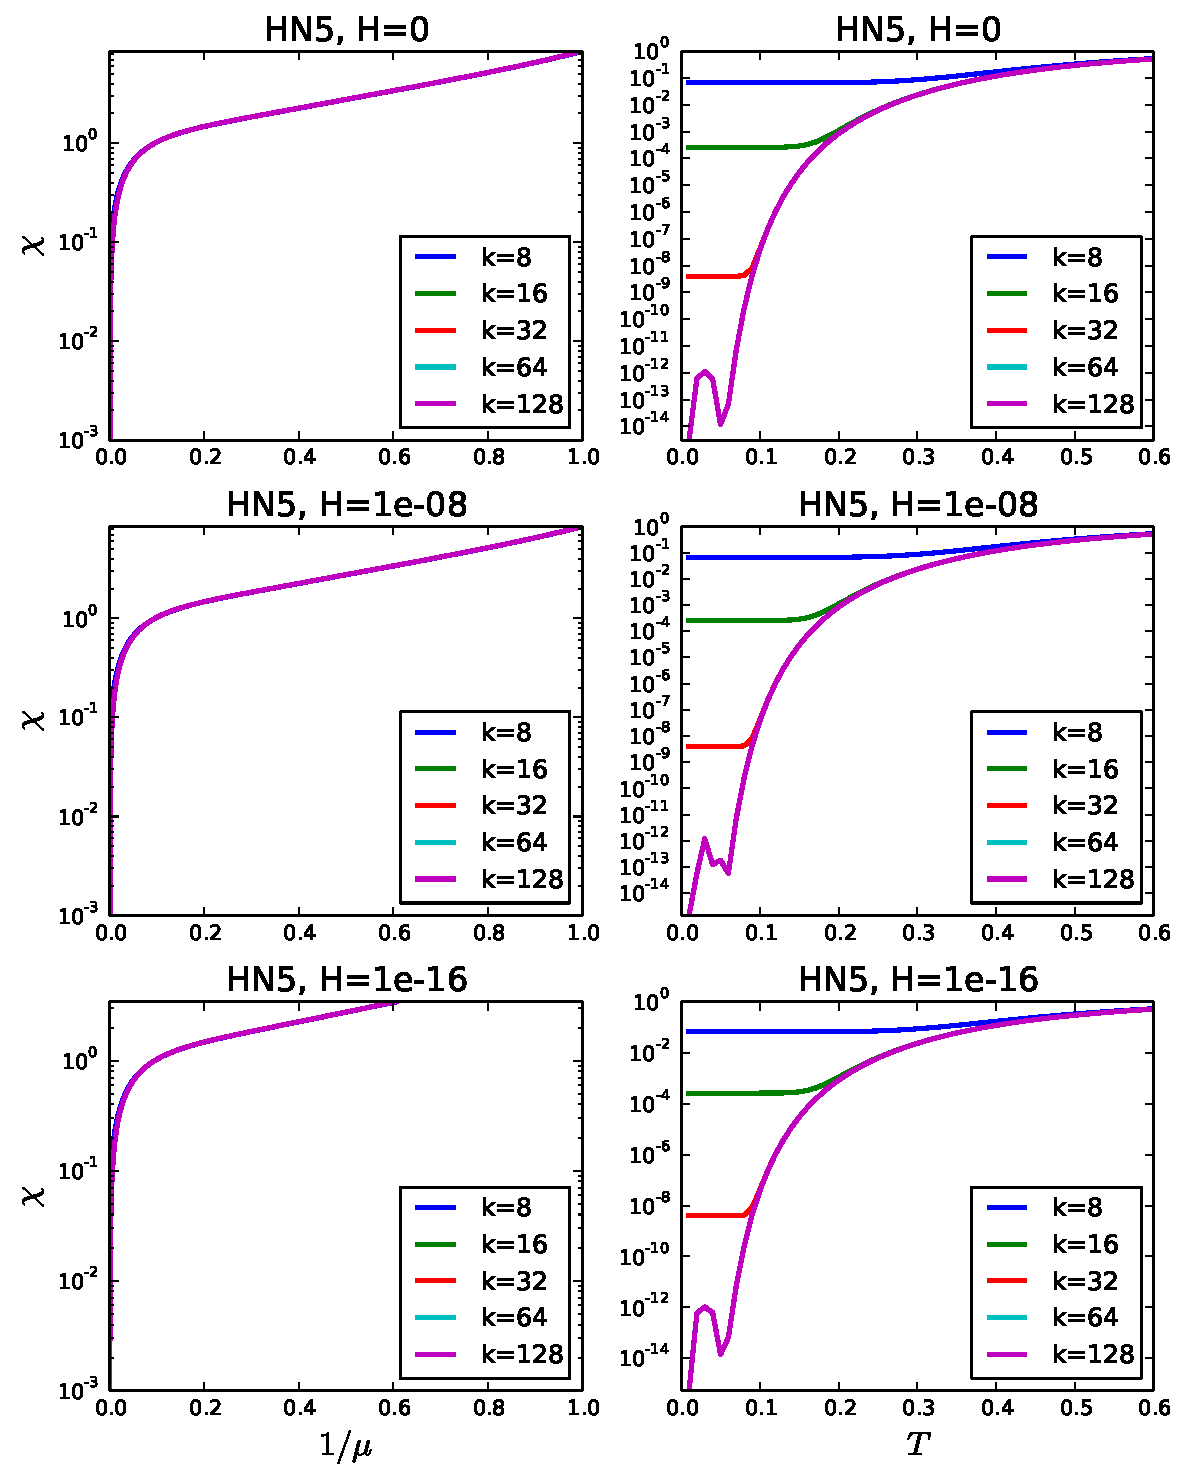
\includegraphics[width=1\columnwidth]{../RG_plots/HN5_XT_rg.pdf}
\caption{HN5 Ising AFM  Susceptibility from RG. The precision of RG is already N[1000].  I may try smaller T step size at low T to improve the accuracy at low $T$.}
\label{fig:h5xrg}
\end{figure}

\subsection{Ising ferromagnet on HNNP}
\label{sec:hnnpfmrg}
The Hamiltonian with magnetic field is
\begin{eqnarray}
\label{eq:hpz0}
 -\beta \mathcal{H}_n &=& K_0 \left(x_{n-2}x_{n-1} + x_{n-1}x_{n} +  x_{n}x_{n+1} +  x_{n+1}x_{n+2}\right) \nonumber \\ 
   && + K_1(x_{n-2}x_{n+1} + x_{n-1}x_{n+2}) + yL_1(x_{n-2} x_{n+2}) \nonumber \\
   && +L_0(x_{n-2}x_{n} + x_{n}x_{n+2})  + 4I \nonumber\\
   && +\frac{H_K}{2}(x_{n-2} + 2x_{n-1}+2x_n+2x_{n+1}+x_{n+2})\nonumber\\
   && +\frac{H_L}{2}(x_{n-2}+2x_n + x_{n+2}) + \frac{H}{2}(x_{n-1}+x_{n+1})\nonumber\\
   && + \frac{T}{2}(x_{n-2}x_{n-1}x_n + x_n x_{n+1} x_{n+2})
\end{eqnarray}
where $y=0$ is for HNNP, and $y=1$ is for HN6. Here we discuss HNNP first, so $y=0$.

Recall that, by fixed point analysis, the transition temperature from stable fixed point to chaotic fixed is $\mu=3$ or $T=1.8205$. We will try to study this temperature more.


\subsubsection{Internal Energy of HNNP}
The ground state energy for $N \rightarrow \infty$ is
\begin{equation}
GS_{HNNP} = -1.48031496062992\dotsc = -\frac{188}{127}
\end{equation}
See the Figure \ref{fig:hperg} and \ref{fig:hpergmc} for results.
\begin{figure}[!htbp]
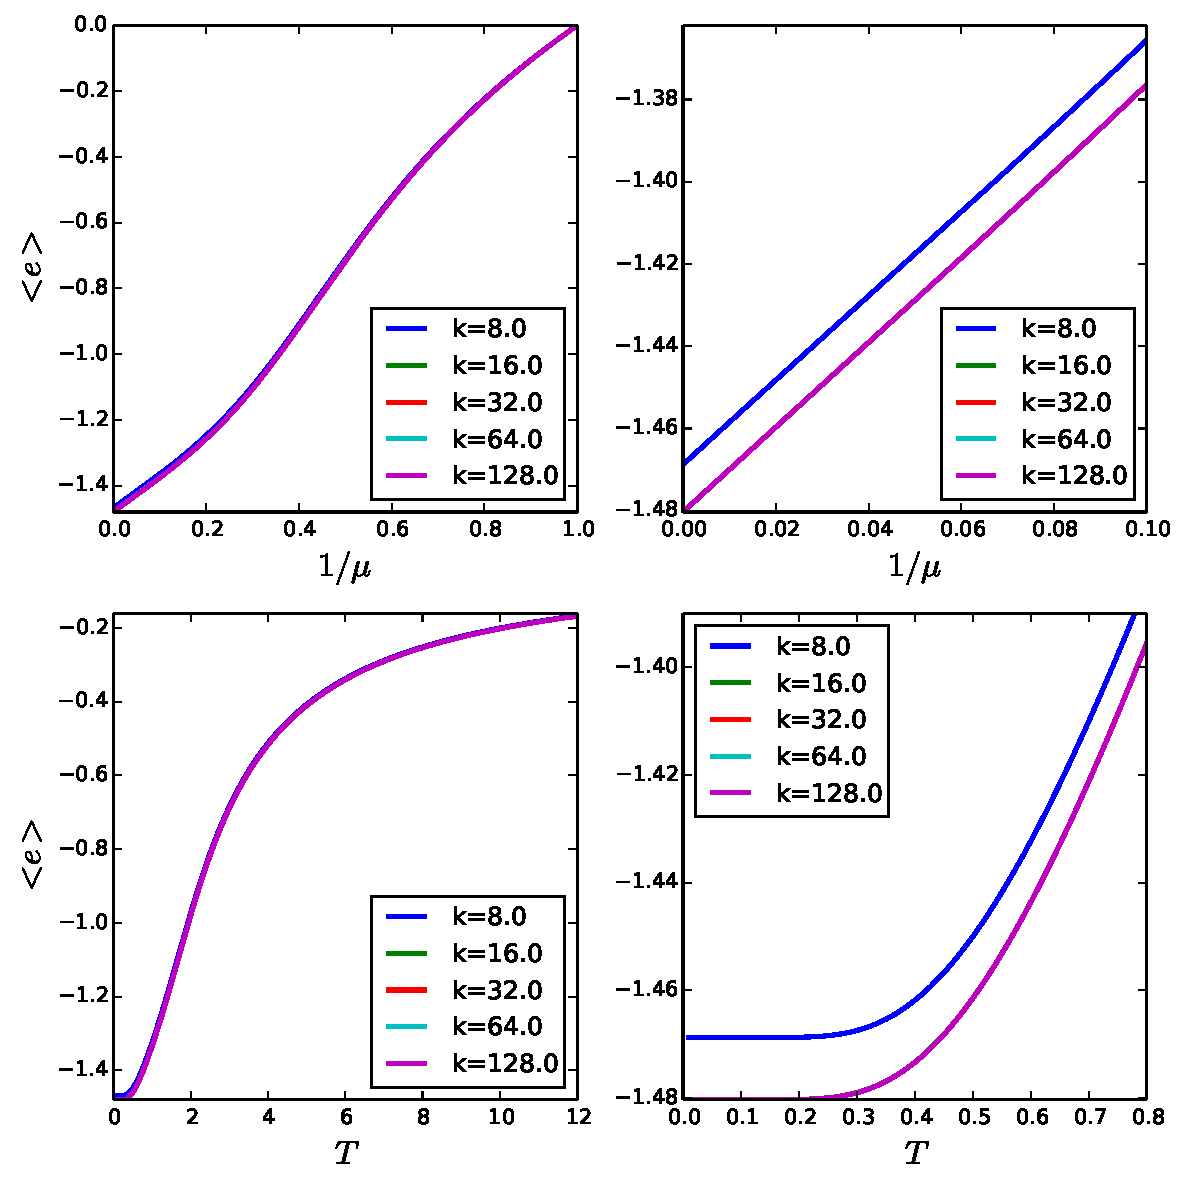
\includegraphics[width=1\columnwidth]{../RG_plots/HNNP_IE_rg.pdf}
\caption{HNNP Ising AFM Internal Energy vs temperature.}
\label{fig:hperg}
\end{figure}

\begin{figure}[!htbp]
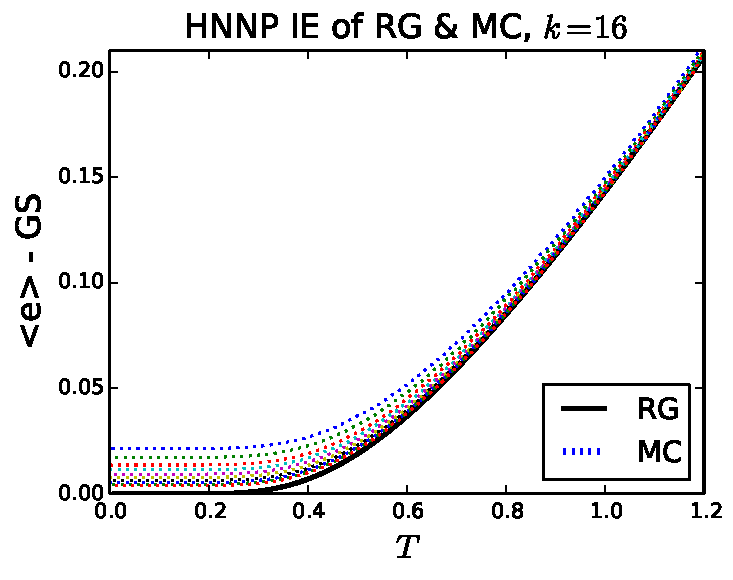
\includegraphics[width=1\columnwidth]{../RG_plots/HNNP_IE_rgmc.pdf}
\caption{HNNP Ising AFM Internal Energy from RG and MC.}
\label{fig:hpergmc}
\end{figure}

\subsubsection{Internal Energy of HN6}
The ground state energy for $N \rightarrow \infty$ is
\begin{equation}
GS_{HNNP} = -1.28571428571428\dotsc = -\frac{9}{7}
\end{equation}
See the Figure \ref{fig:h6erg} and \ref{fig:h6ergmc} for results.
\begin{figure}[!htbp]
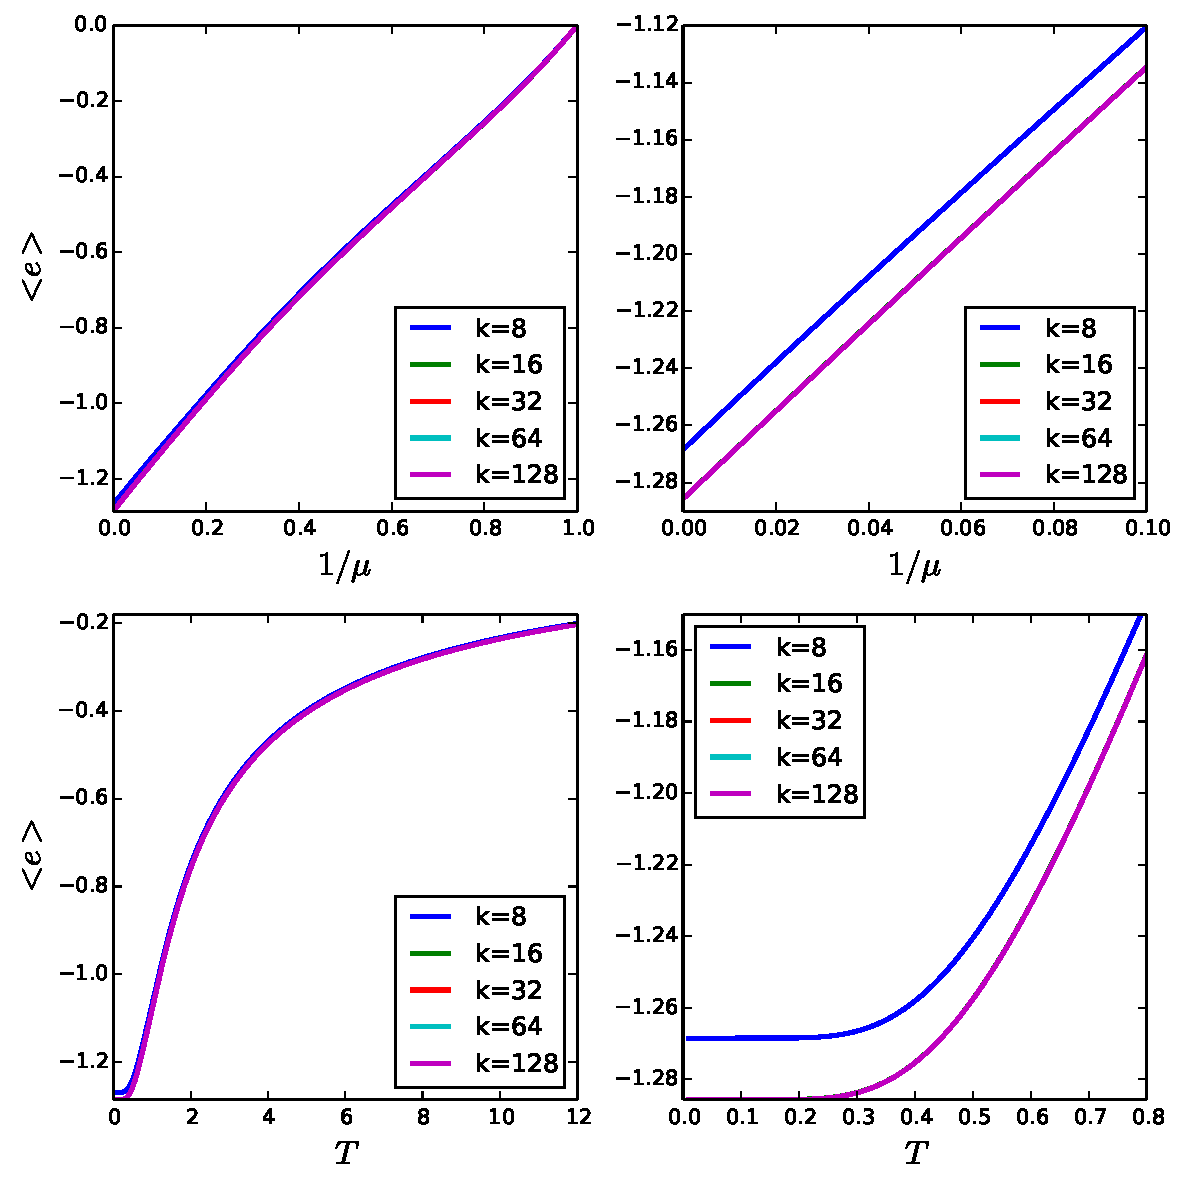
\includegraphics[width=1\columnwidth]{../RG_plots/HN6_IE_rg.pdf}
\caption{HN6 Ising AFM Internal Energy vs temperature.}
\label{fig:h6erg}
\end{figure}

\begin{figure}[!htbp]
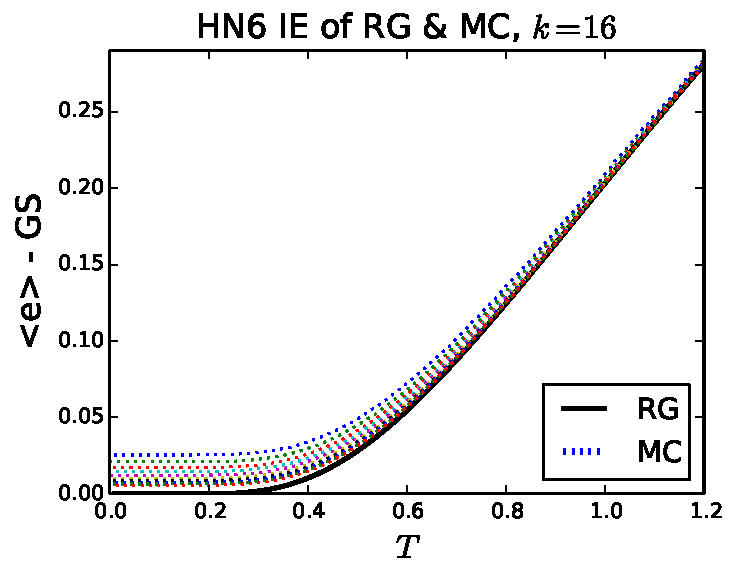
\includegraphics[width=1\columnwidth]{../RG_plots/HN6_IE_rgmc.pdf}
\caption{HN6 Ising AFM Internal Energy from RG and MC.}
\label{fig:h6ergmc}
\end{figure}


\subsubsection{ Magnetization of HNNP}
\textbf{\emph{Magnetization vs. big H}}\\
This part is to learn how $<m>$ changes with $H$, which shows a different phenomena as shown in Figure \ref{fig:hpmhrg}.
\begin{figure}[!htbp]
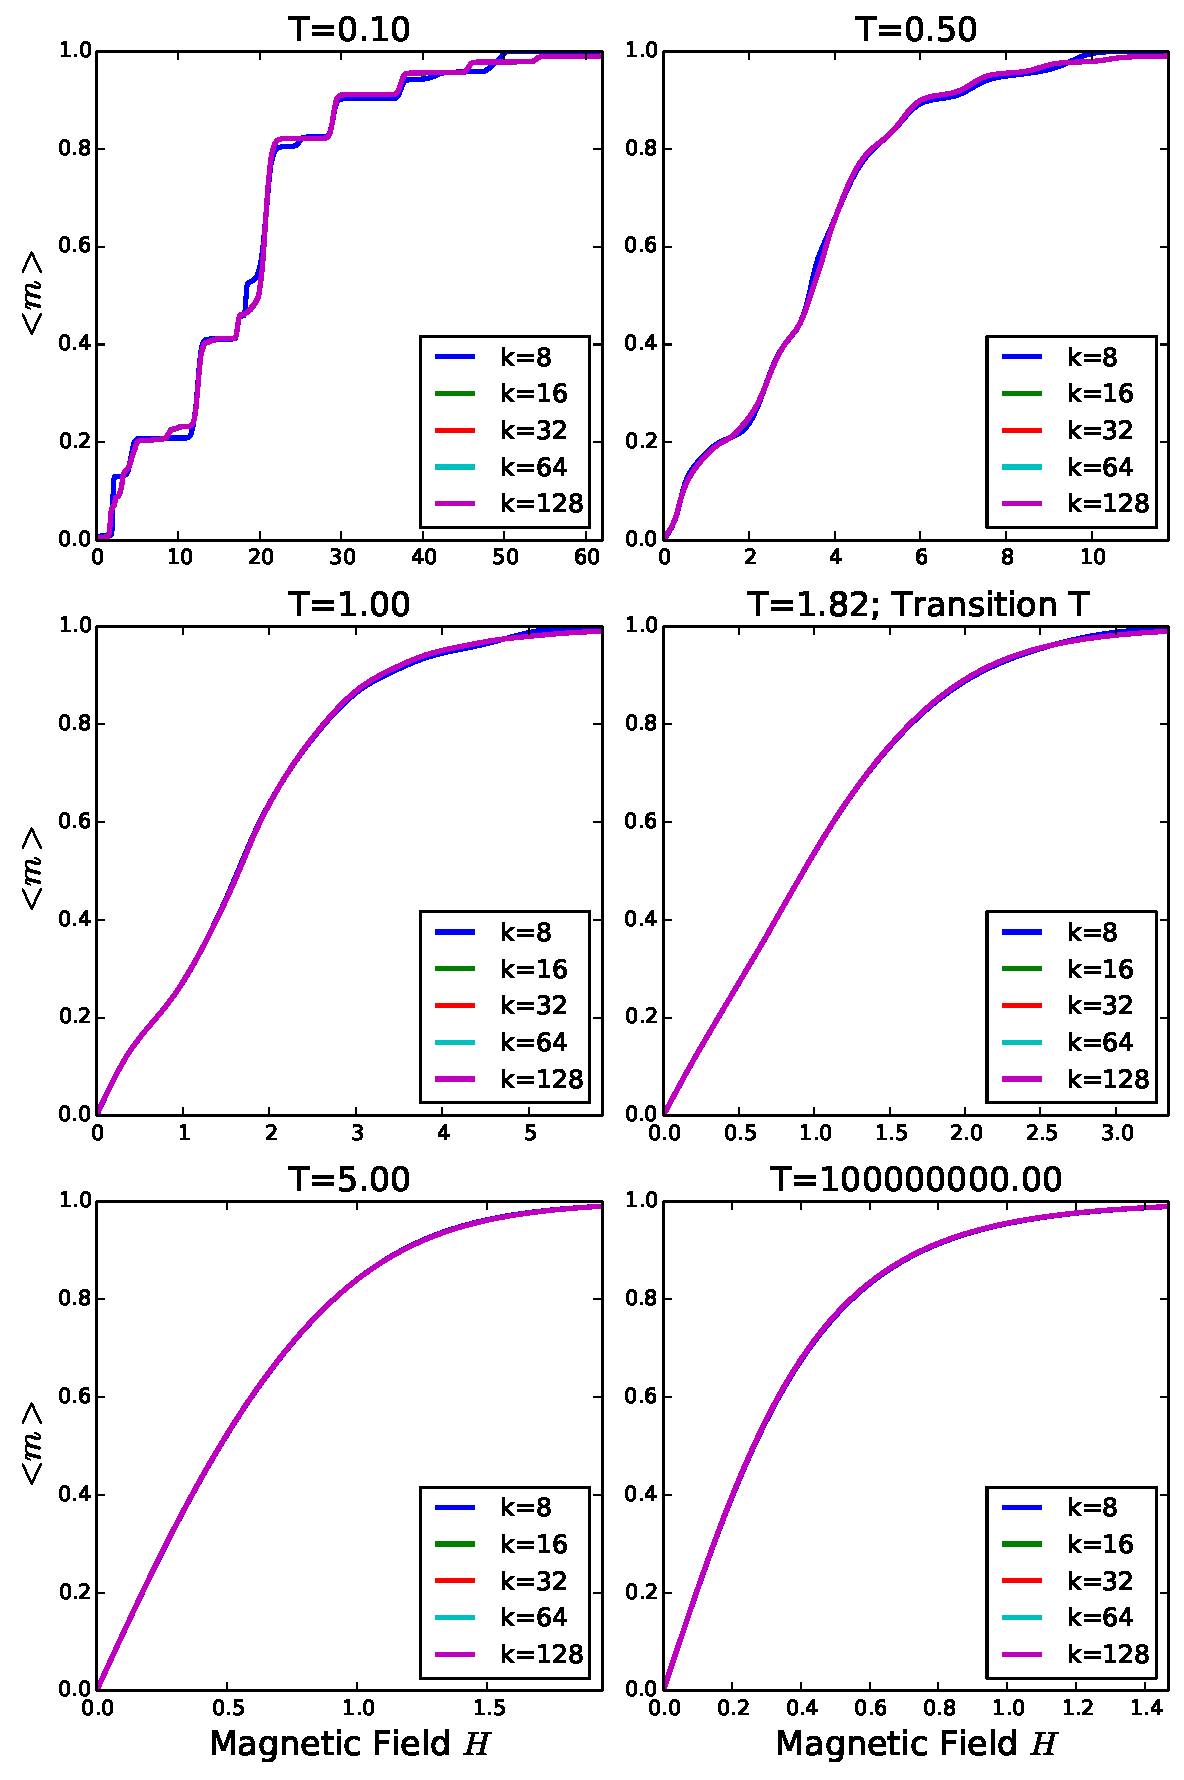
\includegraphics[width=1\columnwidth]{../RG_plots/HNNP_MagH_rg.pdf}
\caption{HNNP Ising AFM magnetization vs magnetic field from RG. $H$ in the RG is actually reduced magnetic field, i.e. $H/T$.}
\label{fig:hpmhrg}
\end{figure}
\\

\textbf{\emph{Magnetization vs. small H}}\\
This part is to learn how $<m>$ changes with small $H$ and how it may break the \'symmetry\'. See Figure \ref{fig:hpmhz2rg} for results.
\begin{figure}[!tbp]
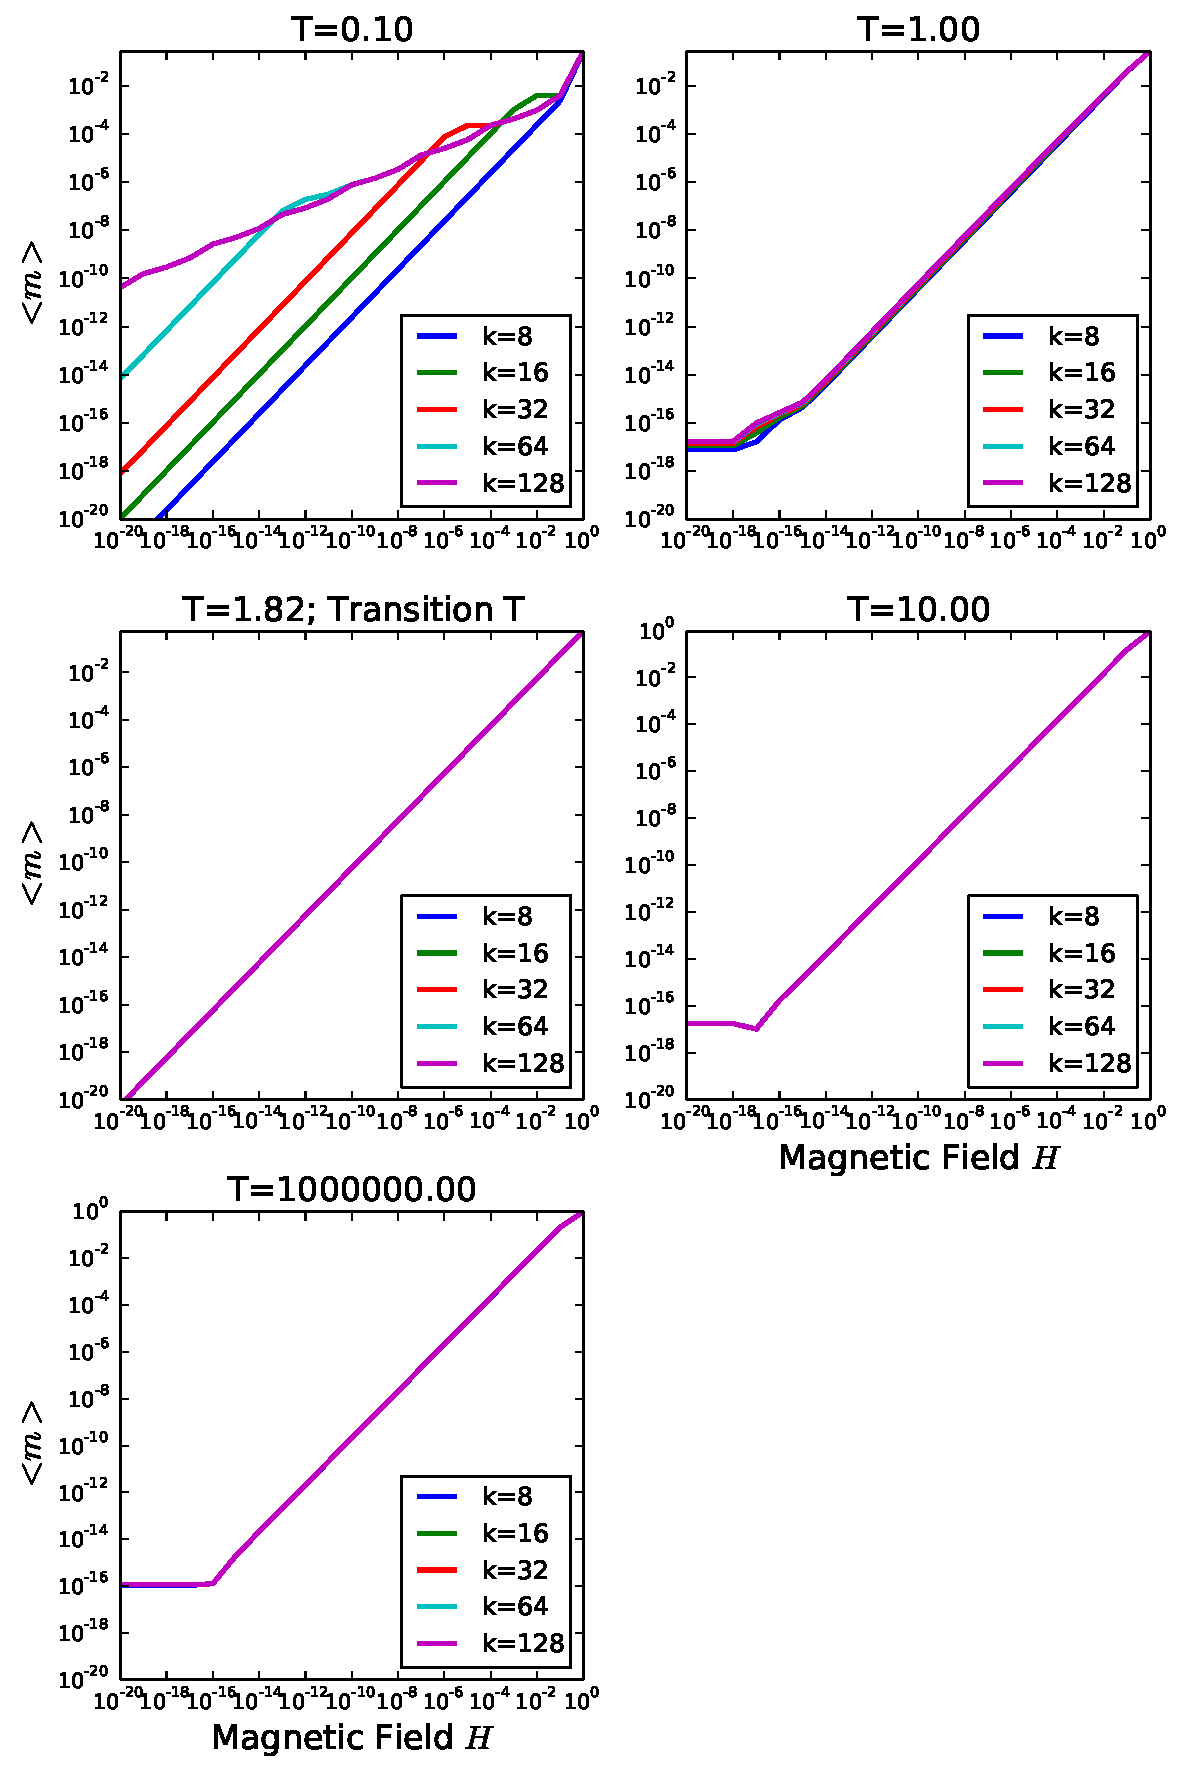
\includegraphics[width=1\columnwidth]{../RG_plots/HNNP_MagHz2_rg.pdf}
\caption{HNNP Ising AFM magnetization vs magnetic field from RG. This part is to learn how $<m>$ changes with small $H$ and how it may break the \'symmetry\'. $H$ in the RG is actually reduced magnetic field, i.e. $H/T$.}
\label{fig:hpmhz2rg}
\end{figure}
\\

\textbf{\emph{Magnetization vs. T}}\\
This part is to learn how $<m>$ changes with small $H$ and how it may break the \'symmetry\'. See Figure \ref{fig:hpmtrg} for results.
\begin{figure}[!tbp]
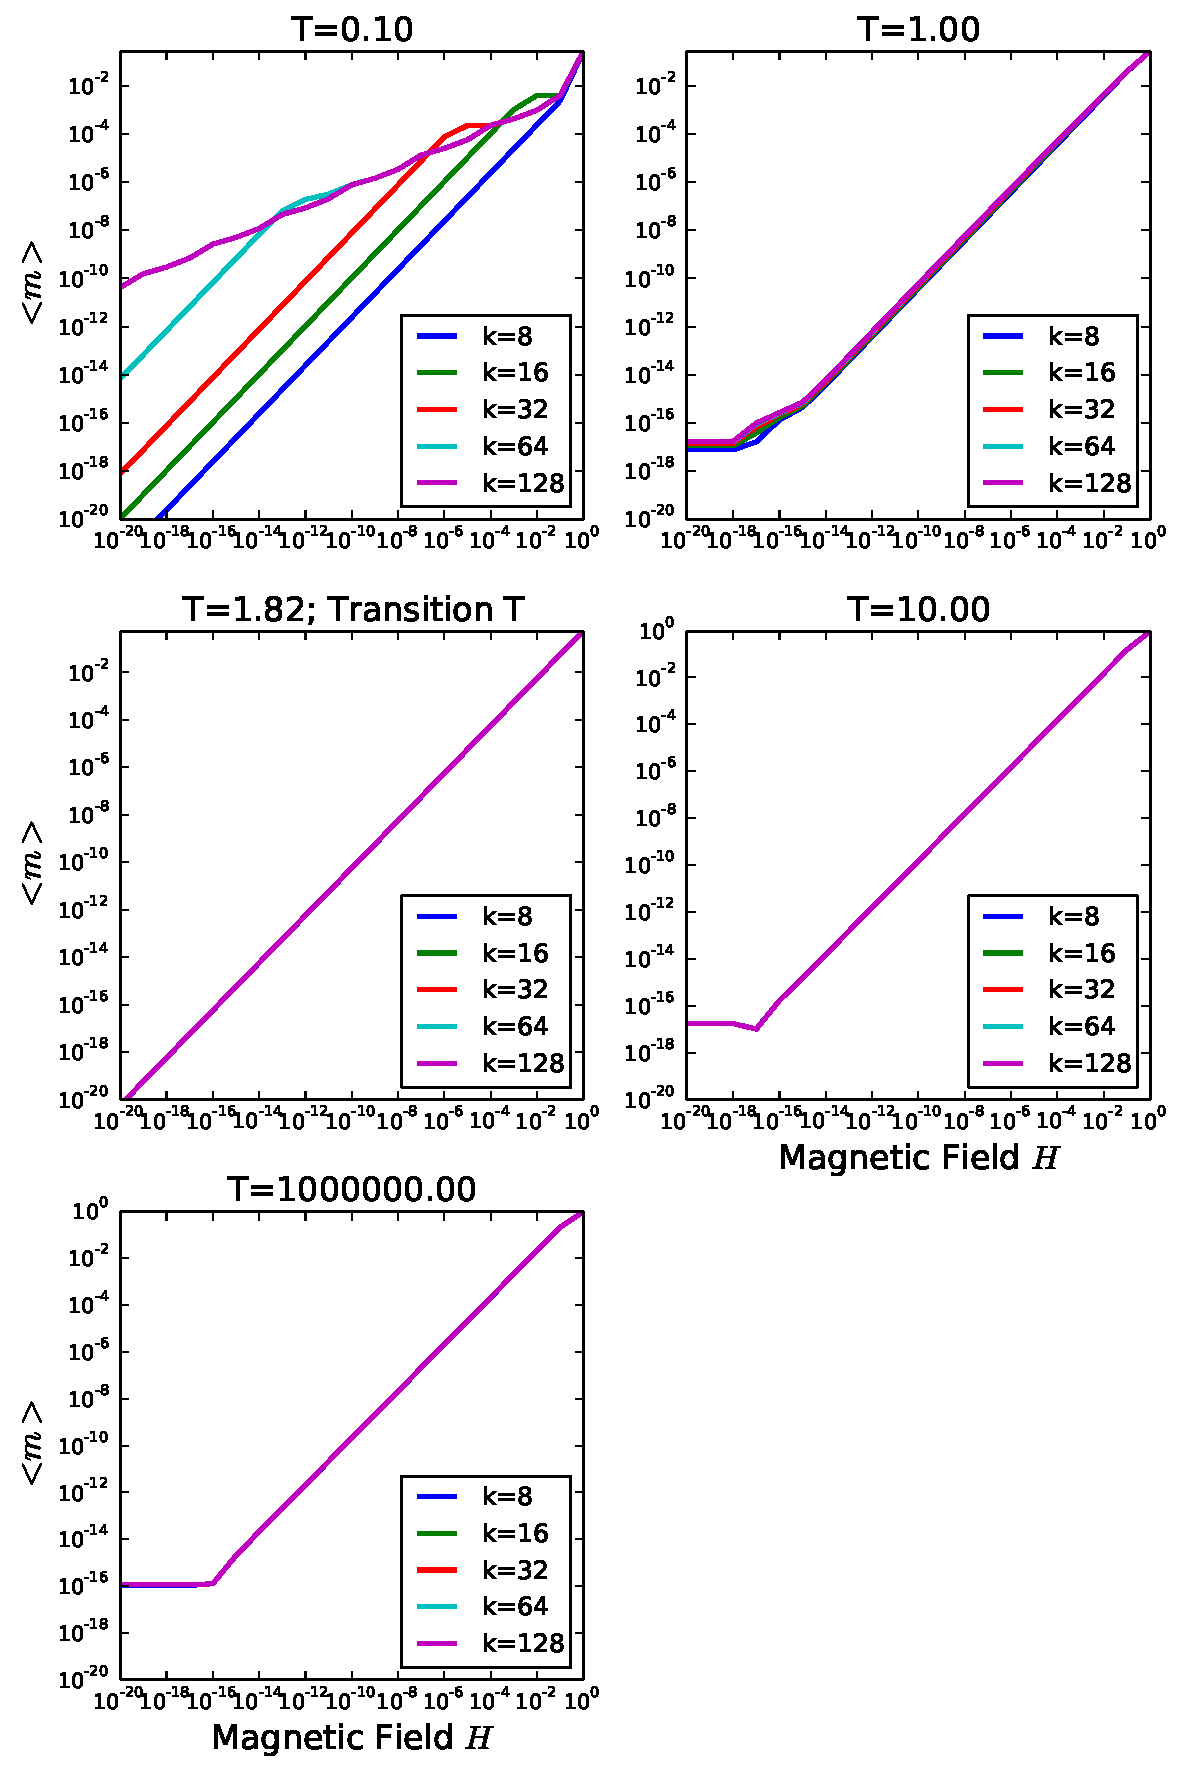
\includegraphics[width=1\columnwidth]{../RG_plots/HNNP_MagHz2_rg.pdf}
\caption{HNNP Ising AFM magnetization vs temperature from RG at different $H$.}
\label{fig:hpmtrg}
\end{figure}


\subsubsection{Specific Heat of HNNP}
See Figure \ref{fig:hpcvrg} for results.

\begin{figure}[!tbp]
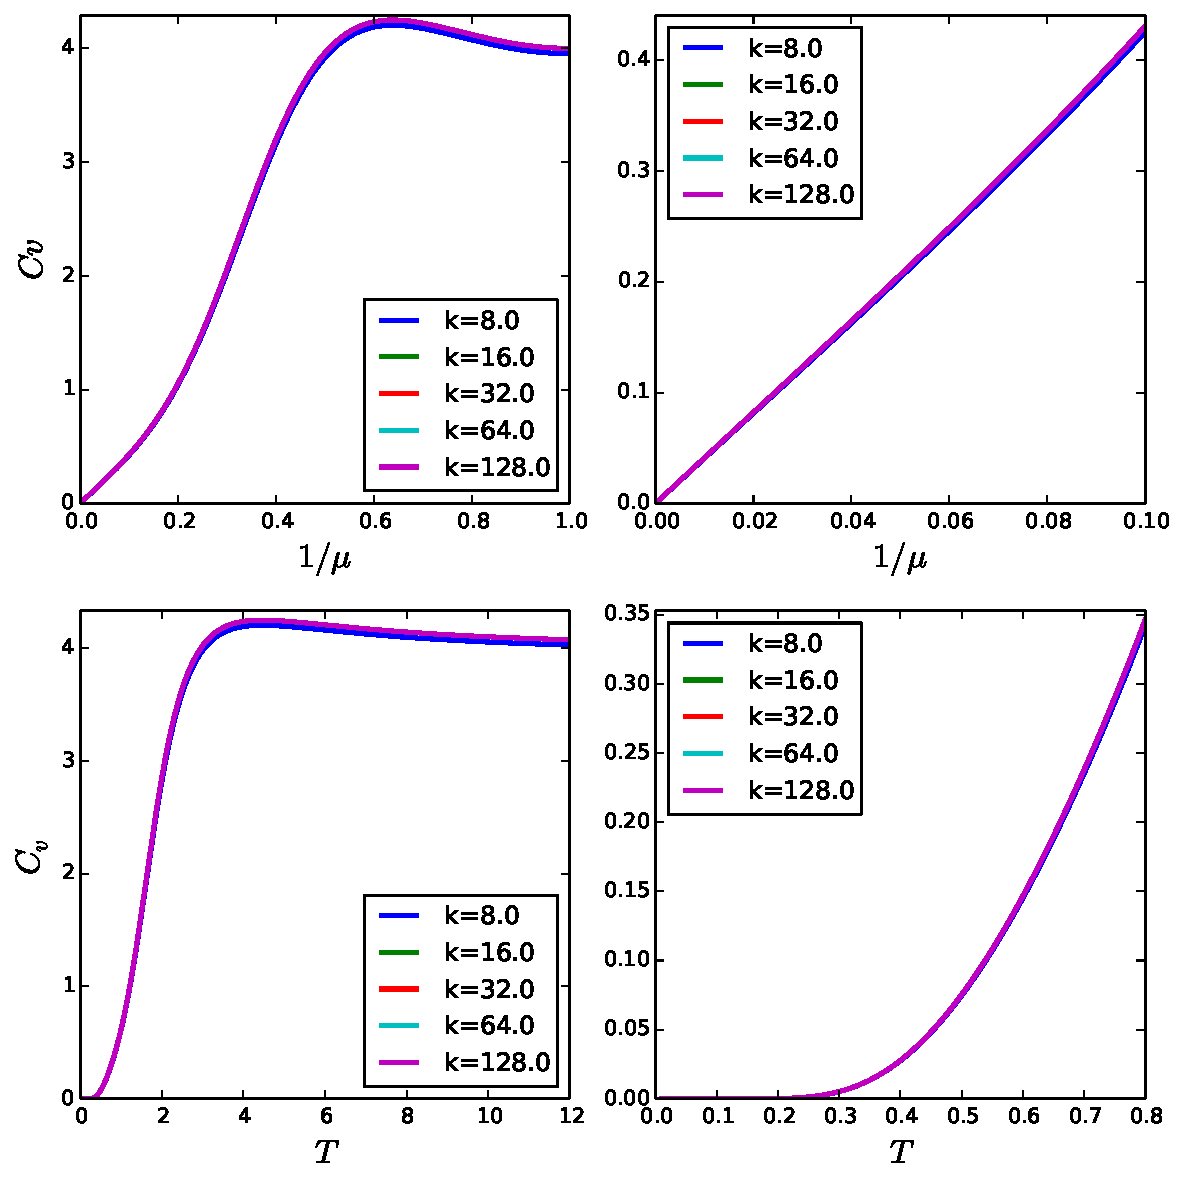
\includegraphics[width=1\columnwidth]{../RG_plots/HNNP_Cv_rg_v2.pdf}
\caption{HNNP Ising AFM Specific Heat from RG.}
\label{fig:hpcvrg}
\end{figure}


\subsubsection{Specific Heat of HN6}
See Figure \ref{fig:h6cvrg} for results.
\begin{figure}[!tbp]
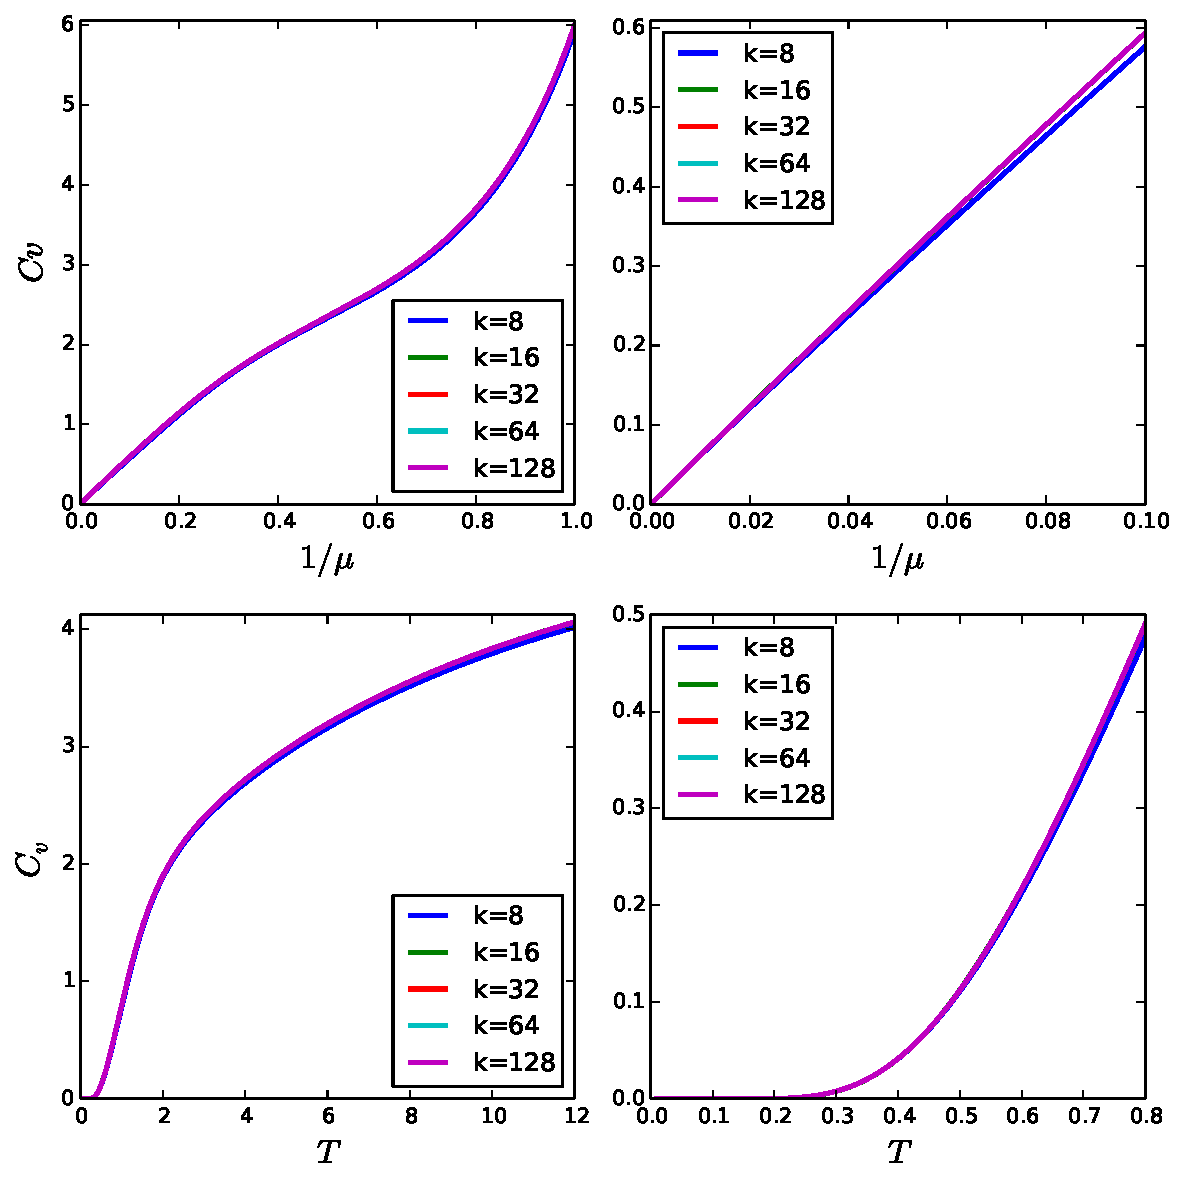
\includegraphics[width=1\columnwidth]{../RG_plots/HN6_Cv_rg.pdf}
\caption{HN6 Ising AFM Specific Heat from RG. }
\label{fig:h6cvrg}
\end{figure}


\subsubsection{Susceptibility of HNNP}
See Figure \ref{fig:hpxrg} for results.
\begin{figure*}[!htbp]
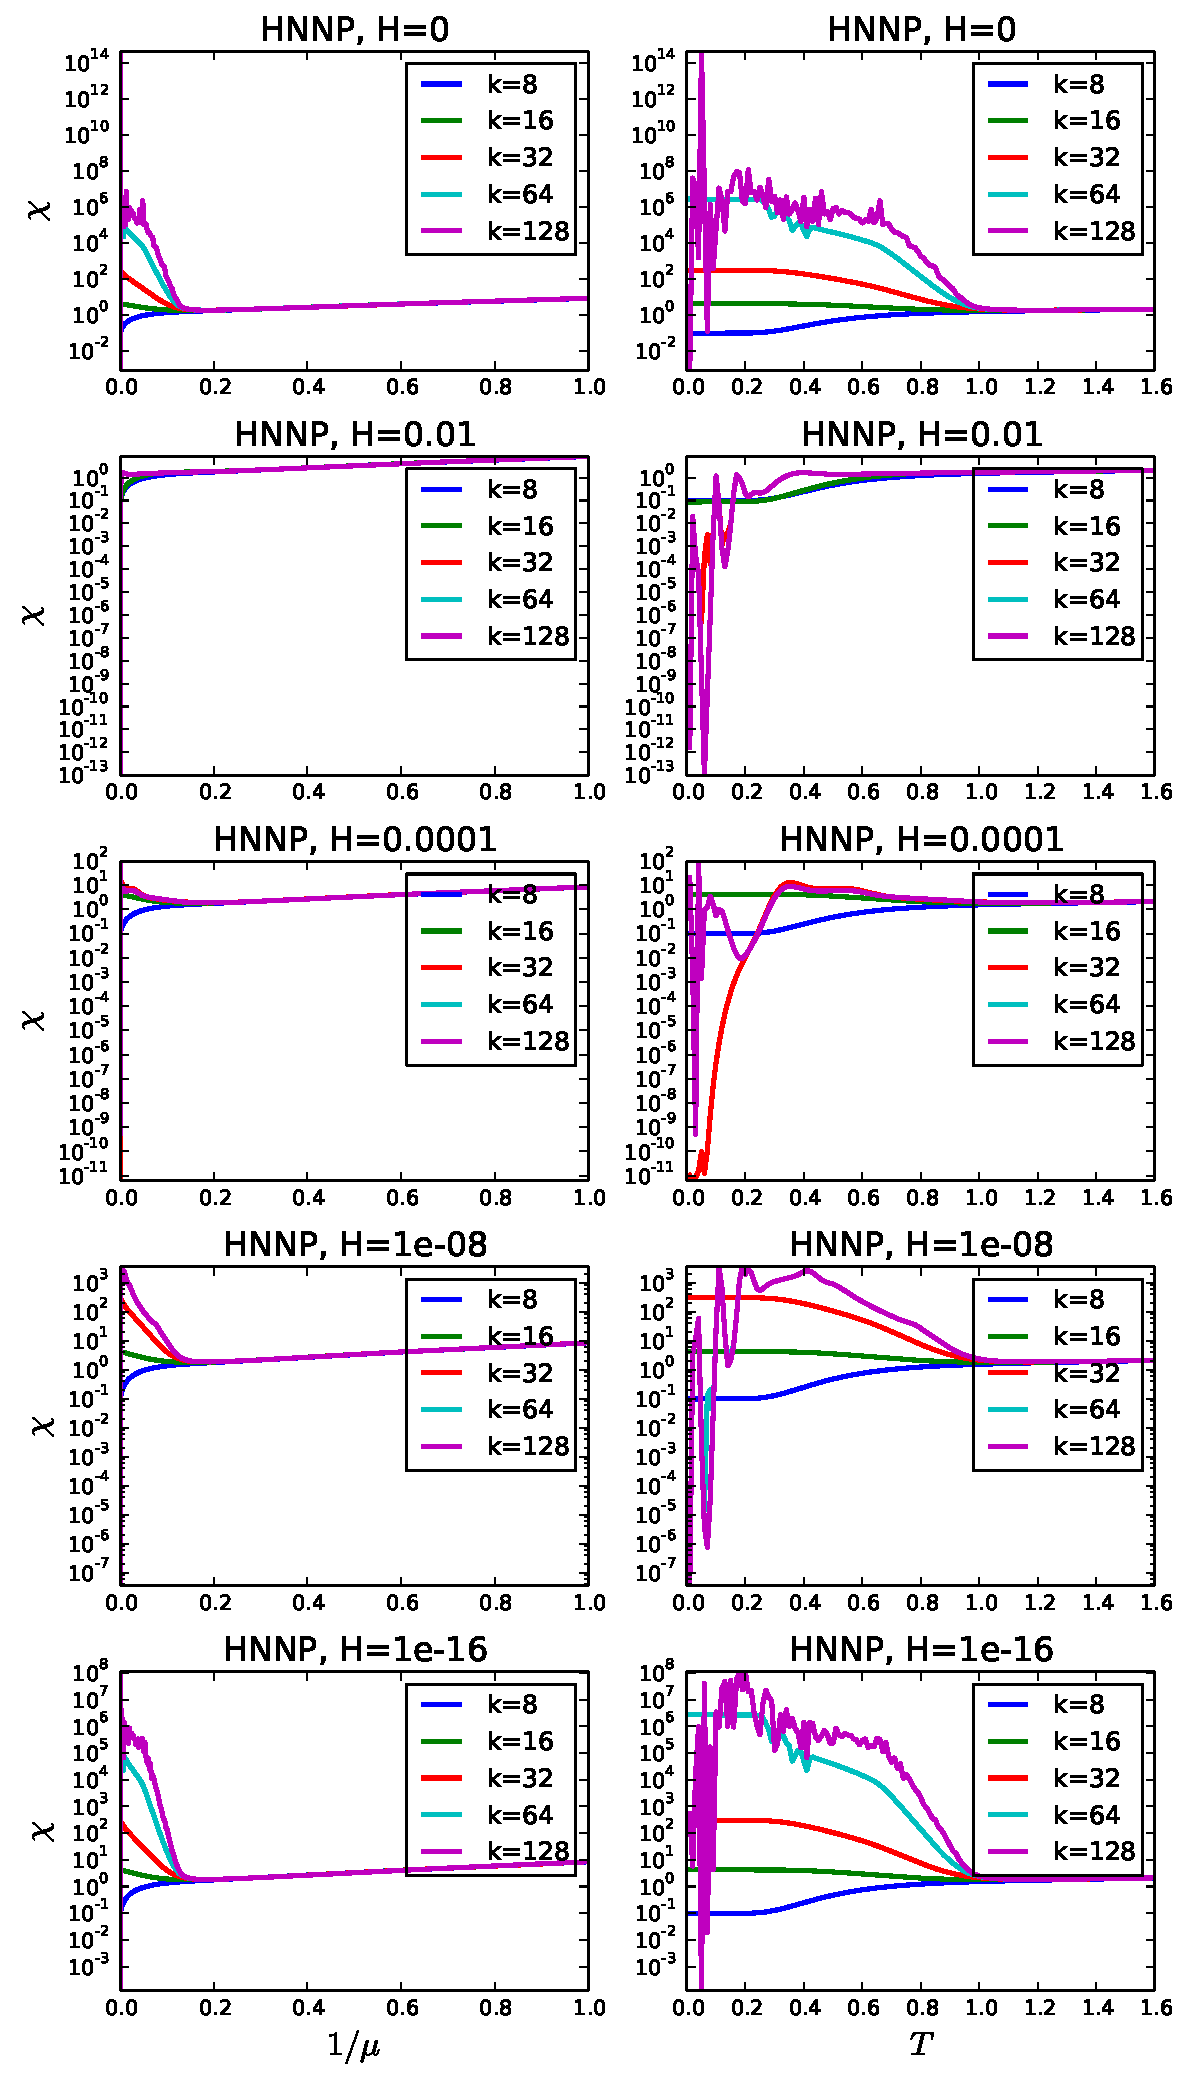
\includegraphics[width=1.5\columnwidth]{../RG_plots/HNNP_XT_rg.pdf}
\caption{HNNP Ising AFM  Susceptibility from RG. The precision of RG is already N[1000].  I may try smaller T step size at low T to improve the accuracy at low $T$.}
\label{fig:hpxrg}
\end{figure*}

\subsubsection{Susceptibility of HN6}
See Figure \ref{fig:h6xrg} for results.
\begin{figure*}[!htbp]
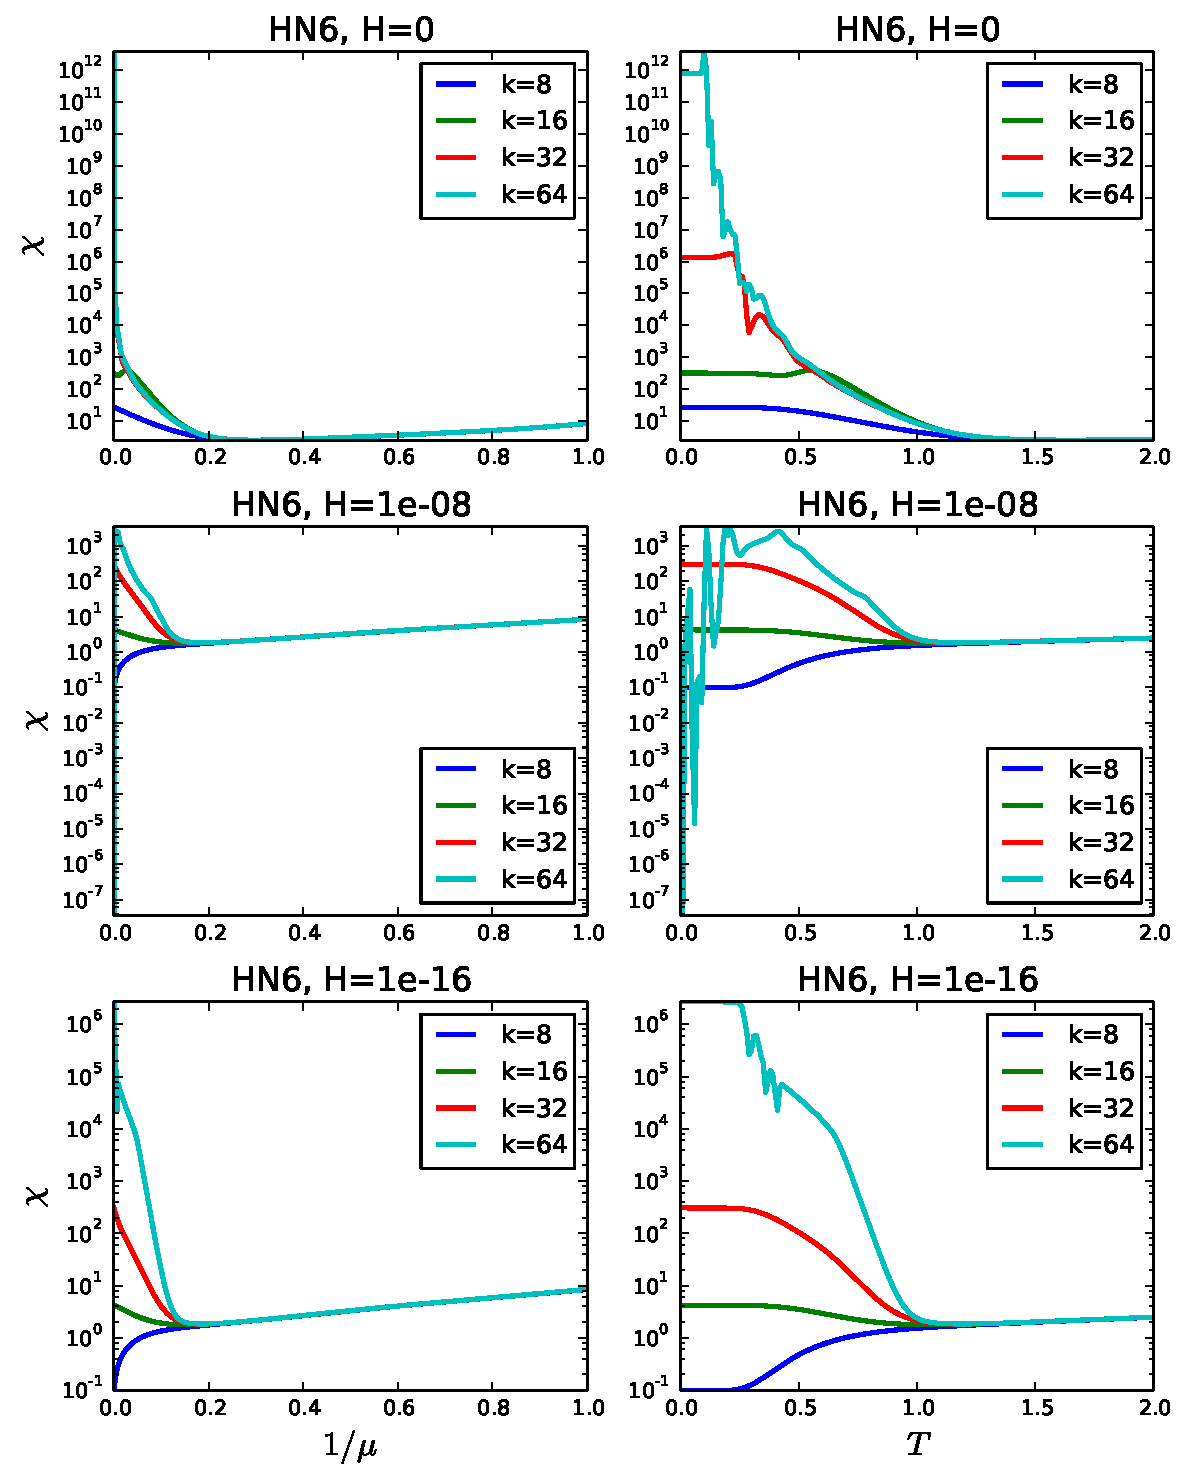
\includegraphics[width=1.5\columnwidth]{../RG_plots/HN6_XT_rg.pdf}
\caption{HN6 Ising AFM  Susceptibility from RG.}
\label{fig:h6xrg}
\end{figure*}


%\bibliographystyle{apsrev4-1}
%\bibliography{Jamming}
\bibliography{cheng}

\end{document}
